% ══════════════════════════════════════════════════════════════════════════
% Research Proposal: Continual Learning and Reinforcement-Learning-Driven
%                    Autonomous Response for Adversarially Robust NIDS
% ══════════════════════════════════════════════════════════════════════════
\documentclass[12pt,a4paper]{article}

% ── Fonts & encoding ────────────────────────────────────────────────────
\usepackage[T1]{fontenc}
\usepackage[utf8]{inputenc}
\usepackage{mathpazo}          % Palatino roman + math
\usepackage[scaled=0.88]{helvet}
\usepackage{microtype}

% ── Layout ──────────────────────────────────────────────────────────────
\usepackage[
  top=25mm, bottom=25mm, left=28mm, right=28mm
]{geometry}
\usepackage{setspace}
\onehalfspacing
\setlength{\parindent}{0pt}
\setlength{\parskip}{6pt}

% ── Headers / footers ──────────────────────────────────────────────────
\usepackage{fancyhdr}
\pagestyle{fancy}
\fancyhf{}
\renewcommand{\headrulewidth}{0.4pt}
\fancyhead[L]{\small\textit{Research Proposal}}
\fancyhead[R]{\small\textit{RobustIDPS.ai}}
\fancyfoot[C]{\thepage}

% ── Figures, maths, tables ─────────────────────────────────────────────
\usepackage{amsmath,amssymb,amsthm}
\usepackage{tikz}
\usetikzlibrary{arrows.meta,positioning,shapes.geometric,calc,fit}
\usepackage{pgfplots}
\pgfplotsset{compat=1.18}
\usepackage{booktabs}
\usepackage{tabularx}
\usepackage{enumitem}
\setlist[enumerate]{leftmargin=*, label=\arabic*.}

% ── References & links ─────────────────────────────────────────────────
\usepackage[
  colorlinks=true, linkcolor=blue!60!black,
  citecolor=blue!60!black, urlcolor=blue!50!black
]{hyperref}
\usepackage[numbers,sort&compress]{natbib}

% ── Custom commands ────────────────────────────────────────────────────
\newcommand{\RobustIDPS}{\textsc{RobustIDPS.ai}}
\newcommand{\EWC}{\textsc{EWC}}
\newcommand{\RL}{\textsc{RL}}

% ── Theorem-like environments ──────────────────────────────────────────
\theoremstyle{definition}
\newtheorem{definition}{Definition}[section]
\newtheorem{objective}{Objective}[section]

% ═══════════════════════════════════════════════════════════════════════
\begin{document}

% ── Title page ─────────────────────────────────────────────────────────
\begin{titlepage}
\begin{center}
\vspace*{2cm}

{\LARGE\bfseries Research Proposal}

\vspace{0.8cm}

{\Large Continual Learning and Reinforcement-Learning-Driven\\[4pt]
Autonomous Response for Adversarially Robust\\[4pt]
Network Intrusion Detection Systems}

\vspace{1.5cm}

{\large\textbf{Roger Nick Anaedevha}}\\[4pt]
{\normalsize MSc Candidate, Institute of Cyber-Intelligent Systems (ICIS)\\
National Research Nuclear University MEPhI\\
Moscow, Russian Federation\\
\texttt{roger@robustidps.ai}}

\vspace{1cm}

{\large\textbf{Supervisor:}}\\[4pt]
{\large Alexander Gennadievich Trofimov}\\[4pt]
{\normalsize Associate Professor, Institute of Cyber-Intelligent Systems (ICIS)\\
National Research Nuclear University MEPhI\\
\texttt{agtrofimov@robustidps.ai}}

\vspace{2cm}

{\normalsize\textit{Submitted in partial fulfilment of the requirements for the\\
degree of Master of Science in Cybersecurity and Artificial Intelligence}}

\vspace{1.5cm}
{\normalsize March 2026}
\end{center}
\end{titlepage}

% ── Table of contents ──────────────────────────────────────────────────
\tableofcontents
\newpage

% ═══════════════════════════════════════════════════════════════════════
\section{Introduction}
\label{sec:intro}

Network intrusion detection systems (NIDS) constitute the first line of defence in modern enterprise security architectures.
Traditional signature-based systems such as Suricata and Snort rely on predefined rule sets that must be manually curated and cannot generalise to novel attack variants.
Machine-learning-based approaches, including the seven-method surrogate ensemble deployed in \RobustIDPS{}, achieve substantially higher detection rates, yet they share a critical limitation: once trained, the model parameters remain static.

In production environments, network traffic distributions evolve continuously.
New application protocols emerge, user behaviour shifts, and adversaries adapt their tactics.
This phenomenon, known as \emph{distribution shift} or \emph{concept drift}, causes the accuracy of fixed-weight classifiers to degrade over time.
Periodic full retraining is computationally expensive, operationally disruptive, and may itself introduce regressions on previously well-classified attack families.

Concurrently, detection without response constitutes only half the defensive mission.
Current systems generate alerts that human analysts must triage, a bottleneck that becomes untenable at scale.
An autonomous response capability that selects and executes mitigation actions, subject to configurable safety constraints, would close the loop between detection and remediation.

This proposal presents a unified research programme that addresses both limitations.
The first component introduces \emph{continual learning} via Elastic Weight Consolidation (\EWC{}) and experience replay, enabling the IDS to adapt incrementally to new traffic without catastrophic forgetting.
The second component designs a \emph{reinforcement learning} agent that maps detection outputs to mitigation actions such as rate limiting, connection resets, and firewall rule injection, trained under a safety-constrained Markov decision process.


% ═══════════════════════════════════════════════════════════════════════
\section{Definitions}
\label{sec:definitions}

\begin{definition}[Continual Learning]
A training paradigm in which a model sequentially learns from a stream of tasks $\mathcal{T}_1, \mathcal{T}_2, \ldots, \mathcal{T}_T$ without access to the full joint dataset, while maintaining performance on all previously encountered tasks.
\end{definition}

\begin{definition}[Catastrophic Forgetting]
The tendency of neural networks trained via gradient descent to lose performance on task $\mathcal{T}_i$ when subsequently optimised on task $\mathcal{T}_{j}$ ($j > i$), owing to unconstrained overwriting of parameters important for earlier tasks.
\end{definition}

\begin{definition}[Elastic Weight Consolidation]
A regularisation technique that adds a quadratic penalty to the loss function during fine-tuning on new data:
\begin{equation}
\mathcal{L}_{\text{EWC}} = \mathcal{L}_{\text{new}}(\theta) + \frac{\lambda}{2} \sum_{k} F_k \left(\theta_k - \theta_k^{*}\right)^2
\label{eq:ewc}
\end{equation}
where $F_k$ is the $k$-th diagonal element of the Fisher Information Matrix computed on the previous task, $\theta_k^{*}$ is the parameter value after training on that task, and $\lambda$ controls the strength of consolidation.
\end{definition}

\begin{definition}[Experience Replay Buffer]
A bounded memory $\mathcal{B}$ of size $M$ that stores representative input--label pairs $(x_i, y_i)$ from past tasks.
During training on new data, mini-batches are formed by mixing current-task samples with uniformly sampled replay elements, yielding $\hat{\mathcal{D}} = \mathcal{D}_{\text{new}} \cup \text{Sample}(\mathcal{B}, m)$.
\end{definition}

\begin{definition}[Distribution Shift (Concept Drift)]
A change in the joint distribution $P(X, Y)$ between the training environment and the deployment environment, which can manifest as covariate shift ($P(X)$ changes), prior probability shift ($P(Y)$ changes), or concept shift ($P(Y|X)$ changes).
\end{definition}

\begin{definition}[Constrained Markov Decision Process]
A tuple $(\mathcal{S}, \mathcal{A}, P, R, C, d_0, \gamma)$ where $\mathcal{S}$ is the state space, $\mathcal{A}$ the action space, $P$ the transition kernel, $R$ the reward function, $C: \mathcal{S} \times \mathcal{A} \to \mathbb{R}$ is a cost function encoding safety constraints, $d_0$ the initial state distribution, and $\gamma$ the discount factor.
The agent maximises $\mathbb{E}[\sum_t \gamma^t R(s_t, a_t)]$ subject to $\mathbb{E}[\sum_t \gamma^t C(s_t, a_t)] \leq \epsilon$.
\end{definition}

\begin{definition}[Autonomous Response Policy]
A mapping $\pi: \mathcal{S} \to \Delta(\mathcal{A})$ that, given the current network state (detection outputs, flow metadata, system load), selects a mitigation action from a predefined action set $\mathcal{A} = \{\texttt{MONITOR}, \texttt{RATE\_LIMIT}, \texttt{RESET}, \texttt{BLOCK}, \texttt{QUARANTINE}\}$.
\end{definition}


% ═══════════════════════════════════════════════════════════════════════
\section{Research Objectives}
\label{sec:objectives}

\begin{objective}[Continual Adaptation]
Design and implement a continual learning pipeline for the \RobustIDPS{} seven-branch surrogate ensemble that enables incremental model updates from new labelled traffic captures while bounding the maximum accuracy regression on any previously learned attack class to no more than 2 percentage points.
\end{objective}

\begin{objective}[Forgetting Quantification]
Develop a rigorous evaluation protocol that measures backward transfer (forgetting), forward transfer (generalisation), and overall plasticity--stability trade-off across at least five sequential task splits derived from the CIC-IoT-2023, CSE-CIC-IDS2018, and UNSW-NB15 benchmarks.
\end{objective}

\begin{objective}[Drift Detection]
Implement an online drift detector that monitors the statistical divergence between the model's training distribution and incoming traffic, triggering update recommendations when the divergence exceeds a calibrated threshold.
\end{objective}

\begin{objective}[RL Response Agent]
Formulate the automated response problem as a Constrained MDP and train a reinforcement learning agent that selects mitigation actions to minimise expected damage, subject to a safety policy that bounds the false-positive blocking rate below 0.1\%.
\end{objective}

\begin{objective}[Safety Guarantees]
Define and enforce a safety policy that prevents the RL agent from executing high-impact actions (e.g., full IP blocks) without sufficient detection confidence ($\geq 0.95$), ensures human-in-the-loop override capability, and logs all automated actions for audit.
\end{objective}

\begin{objective}[Integration and Deployment]
Integrate both components into the existing \RobustIDPS{} production platform, demonstrating end-to-end operation from live network capture through continual model update through automated mitigation.
\end{objective}


% ═══════════════════════════════════════════════════════════════════════
\section{Background and Related Work}
\label{sec:background}

\subsection{Continual Learning in Neural Networks}

The continual learning literature is broadly organised into three families of approaches.
\emph{Regularisation methods}, exemplified by EWC~\cite{kirkpatrick2017}, Synaptic Intelligence~\cite{zenke2017}, and Memory Aware Synapses~\cite{aljundi2018}, add a penalty term to the loss that discourages changes to parameters deemed important for prior tasks.
\emph{Replay methods} maintain an episodic memory of past samples and interleave them during training; Gradient Episodic Memory (GEM)~\cite{lopezpaz2017} and Averaged GEM~\cite{chaudhry2019} additionally constrain gradient directions to avoid increasing the loss on stored exemplars.
\emph{Architecture methods} allocate dedicated capacity for each task, either by growing the network~\cite{rusu2016} or by masking subsets of weights~\cite{serra2018}.

In the intrusion detection domain, continual learning remains largely unexplored.
A small number of works have applied incremental SVMs and online random forests to network data, but these do not scale to the 34-class, 83-feature space of modern CIC-IoT benchmarks and lack the adversarial robustness considerations central to \RobustIDPS{}.

\subsection{Reinforcement Learning for Network Defence}

The application of RL to automated cyber defence has gained traction through simulation environments such as CyberBattleSim~\cite{cyberbattlesim2021} and FARLAND~\cite{molina2021}.
These works typically model the defender as an RL agent operating in a network graph, selecting patching, isolation, or deception actions.
However, most operate in fully simulated environments with simplified traffic models.

Constrained RL~\cite{altman1999} provides the mathematical framework for incorporating safety requirements directly into the policy optimisation objective, ensuring that the agent's behaviour remains within operationally acceptable bounds even during early exploration.


% ═══════════════════════════════════════════════════════════════════════
\section{Methodology}
\label{sec:methodology}

The proposed system is structured as two tightly coupled modules that share the detection backbone of \RobustIDPS{} (Figure~\ref{fig:architecture}).

\subsection{Module 1: EWC-Based Continual Learning}

\subsubsection{Task Formulation}

Each new batch of labelled network traffic constitutes a \emph{task}.
The system maintains the following persistent state between tasks:

\begin{enumerate}
\item The current model parameters $\theta$.
\item The running diagonal Fisher Information Matrix $\hat{F}$, computed as an exponential moving average across tasks: $\hat{F}^{(t)} = \alpha \hat{F}^{(t-1)} + (1 - \alpha) F^{(t)}$, with $\alpha = 0.5$.
\item The star parameters $\theta^{*}$ stored after each update.
\item An experience replay buffer $\mathcal{B}$ of bounded size $M = 5000$.
\end{enumerate}

\subsubsection{Training Procedure}

Given new data $\mathcal{D}_{\text{new}}$ and the current replay buffer $\mathcal{B}$:

\begin{enumerate}
\item Merge training batches: $\hat{\mathcal{D}} = \mathcal{D}_{\text{new}} \cup \text{Sample}(\mathcal{B}, \min(|\mathcal{B}|, |\mathcal{D}_{\text{new}}|))$.
\item Optimise the composite loss $\mathcal{L} = \mathcal{L}_{\text{CE}}(\hat{\mathcal{D}}; \theta) + \frac{\lambda}{2} \sum_k \hat{F}_k (\theta_k - \theta_k^{*})^2$ using Adam with learning rate $10^{-4}$ for $E$ epochs.
\item Recompute the Fisher diagonal on $\mathcal{D}_{\text{new}}$ and update $\hat{F}$, $\theta^{*}$.
\item Update $\mathcal{B}$ via reservoir sampling.
\item Checkpoint the model and EWC state to disk.
\end{enumerate}

\subsubsection{Drift Detection}

Before committing to an update, the system evaluates the current model on the new data to measure the accuracy gap.
Three regimes are defined:

\begin{center}
\begin{tabular}{lcl}
\toprule
Accuracy on new data & Regime & Action \\
\midrule
$\geq 92\%$ & Stable & Continue monitoring \\
$85\%$--$92\%$ & Monitor & Alert; optional update \\
$< 85\%$ & Drift & Update recommended \\
\bottomrule
\end{tabular}
\end{center}

\subsection{Module 2: RL-Based Autonomous Response}

\subsubsection{State Space}

The state $s_t$ at decision time $t$ comprises:

\begin{enumerate}
\item \textbf{Detection vector}: predicted class probabilities $p \in \mathbb{R}^{34}$ from the IDS model.
\item \textbf{Uncertainty}: epistemic and aleatoric uncertainty from MC Dropout.
\item \textbf{Flow metadata}: source/destination IP, port, protocol, packet count, byte volume, duration.
\item \textbf{Context}: current connection rate to the target IP, number of recent alerts, system CPU and memory utilisation.
\end{enumerate}

The full state vector $s_t \in \mathbb{R}^{d}$ is formed by concatenating these features, with $d \approx 55$.

\subsubsection{Action Space}

The discrete action space $\mathcal{A}$ contains five response levels of increasing severity:

\begin{center}
\begin{tabular}{clp{6cm}}
\toprule
Level & Action & Description \\
\midrule
0 & \texttt{MONITOR} & Log the event; no network intervention \\
1 & \texttt{RATE\_LIMIT} & Throttle traffic from the source IP \\
2 & \texttt{RESET} & Send TCP RST to terminate the connection \\
3 & \texttt{BLOCK} & Inject a temporary firewall rule (e.g., iptables DROP) \\
4 & \texttt{QUARANTINE} & Isolate the source IP from internal network segments \\
\bottomrule
\end{tabular}
\end{center}

\subsubsection{Reward Design}

The reward function balances detection effectiveness against operational disruption:

\begin{equation}
R(s_t, a_t) = \underbrace{w_{\text{det}} \cdot \mathbb{1}[\text{threat mitigated}]}_{\text{detection reward}}
- \underbrace{w_{\text{fp}} \cdot \mathbb{1}[\text{benign blocked}]}_{\text{false positive penalty}}
- \underbrace{w_{\text{sev}} \cdot \text{severity}(a_t)}_{\text{action cost}}
\label{eq:reward}
\end{equation}

where $w_{\text{det}} = 10$, $w_{\text{fp}} = 50$ (heavily penalising false positives), and $w_{\text{sev}} \in \{0, 0.5, 1, 2, 5\}$ scales with action severity.

\subsubsection{Safety Constraints}

The agent operates within a Constrained MDP framework.
The primary constraint bounds the false-positive blocking rate:

\begin{equation}
\mathbb{E}\left[\sum_{t} \gamma^t \mathbb{1}[\text{benign blocked at } t]\right] \leq \epsilon_{\text{fp}}
\end{equation}

Additional hard constraints implemented at the environment level:

\begin{enumerate}
\item Actions at level $\geq 3$ (\texttt{BLOCK}) require detection confidence $\geq 0.95$.
\item \texttt{QUARANTINE} actions are logged and require confirmation if the system is in ``human-in-the-loop'' mode.
\item All actions are recorded in the audit log for forensic review.
\item A global rate limiter prevents the agent from issuing more than 100 blocking actions per minute.
\end{enumerate}

\subsubsection{Training Algorithm}

The response policy is trained using Constrained Policy Optimisation (CPO)~\cite{achiam2017}, which extends Trust Region Policy Optimisation with Lagrangian constraint satisfaction.
Training proceeds in a simulated environment constructed from replayed traffic captures.

\begin{figure}[t]
\centering
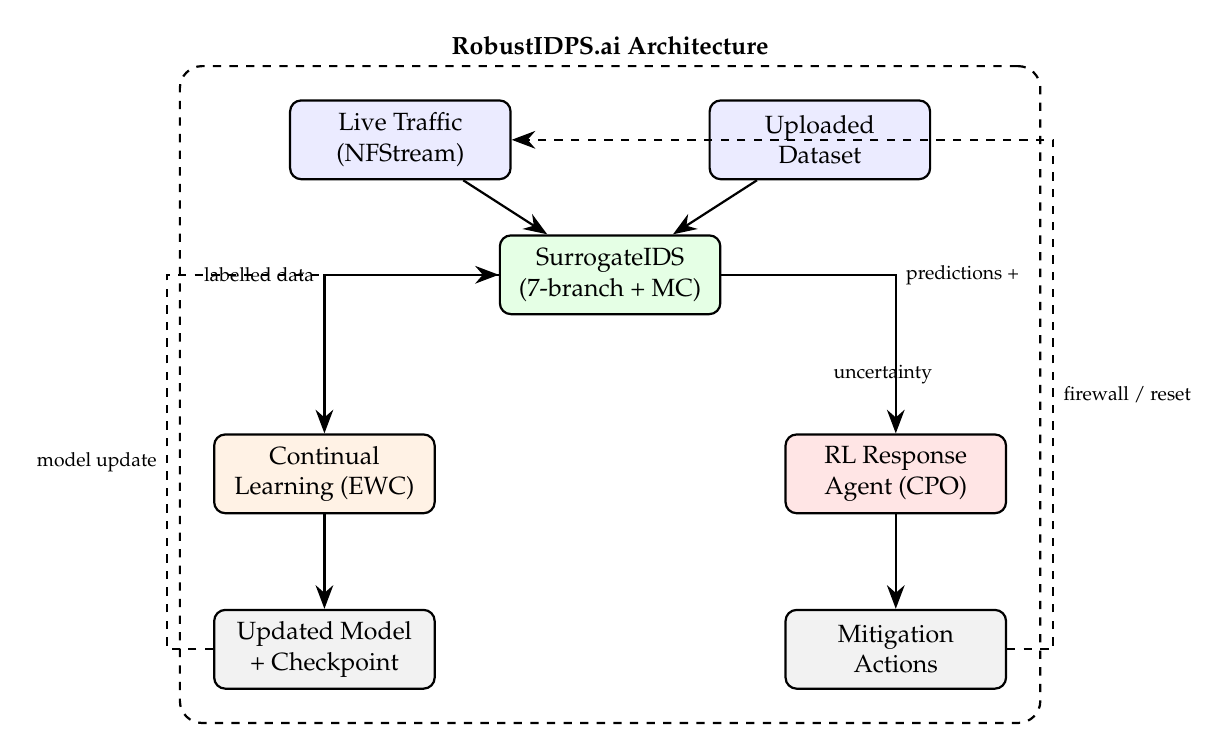
\begin{tikzpicture}[
    node distance=1.2cm and 1.5cm,
    box/.style={draw, rounded corners=4pt, minimum width=2.8cm, minimum height=1cm,
                font=\small, align=center, thick},
    arr/.style={-{Stealth[length=3mm]}, thick},
    darr/.style={-{Stealth[length=3mm]}, thick, dashed},
]
  % Row 1: Data sources
  \node[box, fill=blue!8] (live) {Live Traffic\\(NFStream)};
  \node[box, fill=blue!8, right=2.5cm of live] (upload) {Uploaded\\Dataset};

  % Row 2: Detection
  \node[box, fill=green!10, below=1.2cm of $(live)!0.5!(upload)$] (ids) {SurrogateIDS\\(7-branch + MC)};

  % Row 3: Two modules
  \node[box, fill=orange!10, below left=1.5cm and 0.8cm of ids] (cl) {Continual\\Learning (EWC)};
  \node[box, fill=red!10, below right=1.5cm and 0.8cm of ids] (rl) {RL Response\\Agent (CPO)};

  % Row 4: Outputs
  \node[box, fill=gray!10, below=1.2cm of cl] (ckpt) {Updated Model\\+ Checkpoint};
  \node[box, fill=gray!10, below=1.2cm of rl] (act) {Mitigation\\Actions};

  % Arrows
  \draw[arr] (live) -- (ids);
  \draw[arr] (upload) -- (ids);
  \draw[arr] (ids) -| (cl) node[midway, left, font=\scriptsize] {labelled data};
  \draw[arr] (ids) -| (rl) node[midway, right, font=\scriptsize] {predictions +};
  \node[font=\scriptsize, right=0.2cm] at ($(ids)!0.5!(rl) + (0.7, 0)$) {uncertainty};
  \draw[arr] (cl) -- (ckpt);
  \draw[arr] (rl) -- (act);
  \draw[darr] (ckpt) -- +(-2,0) |- (ids) node[near start, left, font=\scriptsize] {model update};
  \draw[darr] (act) -- +(2,0) |- node[near start, right, font=\scriptsize] {firewall / reset} (live);

  % Bounding box
  \node[draw, dashed, thick, rounded corners=8pt, fit=(live)(upload)(ids)(cl)(rl)(ckpt)(act),
        inner sep=12pt, label={[font=\small\bfseries]above:RobustIDPS.ai Architecture}] {};
\end{tikzpicture}
\caption{Proposed system architecture showing the integration of the continual learning module (left branch) and the RL response agent (right branch) with the existing SurrogateIDS detection backbone.}
\label{fig:architecture}
\end{figure}


% ═══════════════════════════════════════════════════════════════════════
\section{Experimental Design}
\label{sec:experiments}

\subsection{Continual Learning Evaluation}

\subsubsection{Sequential Task Protocol}

The CIC-IoT-2023 dataset (33 attack classes) is partitioned into five temporal splits, each representing a distinct ``deployment period.''
The model is initially trained on Split~1 and then incrementally updated on Splits~2--5.
Evaluation metrics are computed on a held-out test set spanning all five periods.

\begin{center}
\begin{tabular}{ll}
\toprule
Metric & Definition \\
\midrule
Average Accuracy (AA) & $\frac{1}{T}\sum_{t=1}^{T} a_{T,t}$, where $a_{T,t}$ is the accuracy on task $t$ after learning task $T$ \\
Backward Transfer (BWT) & $\frac{1}{T-1}\sum_{t=1}^{T-1}(a_{T,t} - a_{t,t})$; negative BWT = forgetting \\
Forward Transfer (FWT) & $\frac{1}{T-1}\sum_{t=2}^{T}(a_{t,t} - \tilde{a}_t)$; $\tilde{a}_t$ = accuracy of a randomly initialised model on task $t$ \\
\bottomrule
\end{tabular}
\end{center}

\subsubsection{Baselines}

\begin{enumerate}
\item \textbf{Full Retraining}: retrain from scratch on the union of all data seen so far.
\item \textbf{Fine-Tuning}: standard SGD on new data without any regularisation.
\item \textbf{EWC only}: Elastic Weight Consolidation without experience replay.
\item \textbf{EWC + Replay}: the proposed method.
\item \textbf{GEM}: Gradient Episodic Memory for comparison with a constrained-gradient approach.
\end{enumerate}

\subsection{RL Agent Evaluation}

The RL agent is evaluated in a simulation environment that replays recorded traffic with injected attack sequences.
Metrics include:

\begin{enumerate}
\item \textbf{Threat Mitigation Rate}: fraction of true attacks that receive a response action at level $\geq 1$.
\item \textbf{False Positive Block Rate}: fraction of benign flows incorrectly blocked ($a_t \geq 3$).
\item \textbf{Mean Time to Respond}: average latency between detection and action execution.
\item \textbf{Constraint Violation Rate}: fraction of episodes where safety constraints are violated.
\item \textbf{Cumulative Reward}: total discounted reward over evaluation episodes.
\end{enumerate}

\subsubsection{RL Baselines}

\begin{enumerate}
\item \textbf{Rule-Based Policy}: deterministic threshold policy (if confidence $> c$ and severity $\geq s$, apply action level $= f(\text{severity})$).
\item \textbf{Unconstrained PPO}: Proximal Policy Optimisation without safety constraints.
\item \textbf{CPO}: the proposed Constrained Policy Optimisation approach.
\item \textbf{Lagrangian PPO}: PPO with Lagrangian relaxation of constraints.
\end{enumerate}


% ═══════════════════════════════════════════════════════════════════════
\section{Expected Outcomes}
\label{sec:expected}

\subsection{Continual Learning}

\begin{enumerate}
\item The EWC + Replay method is expected to maintain average accuracy within 2 percentage points of the full-retraining upper bound, while requiring less than 10\% of the computational cost.
\item Backward transfer (forgetting) should remain above $-0.02$ across all sequential tasks, compared to $-0.15$ or worse for naive fine-tuning.
\item The drift detection mechanism should achieve an AUC of at least 0.90 on a held-out set of concept-drift scenarios, providing actionable recommendations to operators.
\item The system should demonstrate sub-minute update latency on datasets of up to 50\,000 flows when deployed on a single GPU (Hetzner GPU instance).
\end{enumerate}

\subsection{RL Autonomous Response}

\begin{enumerate}
\item The CPO-trained agent is expected to achieve a threat mitigation rate above 95\% while maintaining the false-positive blocking rate below 0.1\%.
\item Compared to the rule-based baseline, the RL agent should reduce mean time to respond by at least 40\% by learning to preemptively escalate on high-confidence detections.
\item Safety constraint violations during evaluation should be zero or near-zero, demonstrating the effectiveness of constrained optimisation.
\item The agent should generalise across different attack mixes without requiring per-scenario tuning.
\end{enumerate}

\subsection{Integrated System}

\begin{enumerate}
\item End-to-end demonstration: live traffic is captured, classified by the continually updated IDS, and automatically mitigated by the RL agent, all within the \RobustIDPS{} web interface.
\item The continual learning module feeds updated uncertainty estimates to the RL agent, improving its action selection as the detection model adapts.
\item Audit logs provide full traceability of both model updates and automated actions.
\end{enumerate}


% ═══════════════════════════════════════════════════════════════════════
\section{Timeline}
\label{sec:timeline}

\begin{center}
\begin{tabularx}{\textwidth}{lXl}
\toprule
Phase & Activities & Duration \\
\midrule
1. Foundation & Literature review; EWC implementation and unit tests; sequential task protocol design & Months 1--2 \\
2. Continual Learning & Full CL pipeline; drift detection; hyperparameter search ($\lambda$, $M$, $\alpha$); benchmark evaluation & Months 3--4 \\
3. RL Environment & CMDP formulation; simulation environment; reward and safety constraint design & Months 4--5 \\
4. RL Training & CPO implementation; baseline comparisons; safety auditing & Months 5--7 \\
5. Integration & Web UI for CL and RL; live capture integration; end-to-end testing & Months 7--8 \\
6. Evaluation & Comprehensive benchmarks; ablation studies; paper writing & Months 8--10 \\
\bottomrule
\end{tabularx}
\end{center}


% ═══════════════════════════════════════════════════════════════════════
\section{Resource Requirements}
\label{sec:resources}

\begin{enumerate}
\item \textbf{Compute}: Hetzner dedicated GPU server (NVIDIA A100 or equivalent) for RL training and CL experiments.
  Current CPU-only deployment suffices for inference but not for the training loops proposed here.
\item \textbf{Data}: CIC-IoT-2023 (1.6\,M flows, 33 attacks), CSE-CIC-IDS2018 (16\,M flows, 14 attacks), UNSW-NB15 (2.5\,M flows, 9 attacks).
  All datasets are publicly available and already supported by the \RobustIDPS{} feature extraction pipeline.
\item \textbf{Software}: PyTorch 2.x, Stable-Baselines3 with Safety Gymnasium, FastAPI, React.
\end{enumerate}


% ═══════════════════════════════════════════════════════════════════════
\section{Ethical Considerations}
\label{sec:ethics}

The proposed autonomous response capability raises important ethical questions.
All mitigation actions are logged, auditable, and reversible.
The safety policy framework explicitly prevents the system from executing permanent blocks without human confirmation.
The false-positive penalty in the reward function ($w_{\text{fp}} = 50$, five times the detection reward) encodes a strong preference for avoiding harm to legitimate users.
During initial deployment, the system will operate in ``shadow mode,'' logging recommended actions without executing them, to allow operators to validate the policy before granting enforcement authority.


% ═══════════════════════════════════════════════════════════════════════
\section{Conclusion}
\label{sec:conclusion}

This proposal outlines a research programme that extends \RobustIDPS{} in two complementary directions.
Continual learning addresses the fundamental limitation of static model weights in non-stationary network environments, using EWC regularisation and experience replay to preserve previously acquired knowledge while incorporating new traffic patterns.
Reinforcement-learning-driven autonomous response addresses the equally fundamental gap between detection and mitigation, using constrained policy optimisation to ensure that automated actions remain within safe operational bounds.

Together, these components will transform \RobustIDPS{} from a detection-only platform into a fully adaptive, closed-loop intrusion detection and response system, bringing it closer to the vision of a self-healing network defence infrastructure.


% ═══════════════════════════════════════════════════════════════════════
\begin{thebibliography}{20}
\bibitem{kirkpatrick2017}
J.~Kirkpatrick et~al., ``Overcoming catastrophic forgetting in neural networks,''
\textit{Proc. Natl. Acad. Sci.}, vol.~114, no.~13, pp.~3521--3526, 2017.

\bibitem{zenke2017}
F.~Zenke, B.~Poole, and S.~Ganguli, ``Continual learning through synaptic intelligence,''
in \textit{Proc. ICML}, 2017, pp.~3987--3995.

\bibitem{aljundi2018}
R.~Aljundi, F.~Babiloni, M.~Elhoseiny, M.~Rohrbach, and T.~Tuytelaars,
``Memory aware synapses: Learning what (not) to forget,''
in \textit{Proc. ECCV}, 2018, pp.~139--154.

\bibitem{lopezpaz2017}
D.~Lopez-Paz and M.~Ranzato, ``Gradient episodic memory for continual learning,''
in \textit{Proc. NeurIPS}, 2017, pp.~6467--6476.

\bibitem{chaudhry2019}
A.~Chaudhry, M.~Ranzato, M.~Rohrbach, and M.~Elhoseiny,
``Efficient lifelong learning with A-GEM,''
in \textit{Proc. ICLR}, 2019.

\bibitem{rusu2016}
A.~A.~Rusu et~al., ``Progressive neural networks,''
\textit{arXiv preprint arXiv:1606.04671}, 2016.

\bibitem{serra2018}
J.~Serra, D.~Suris, M.~Miron, and A.~Karatzoglou,
``Overcoming catastrophic forgetting with hard attention to the task,''
in \textit{Proc. ICML}, 2018, pp.~4548--4557.

\bibitem{cyberbattlesim2021}
Microsoft Defender Research Team, ``CyberBattleSim,''
\textit{GitHub repository}, 2021.

\bibitem{molina2021}
A.~Molina-Markham et~al., ``Network defence is not a game,''
in \textit{Proc. AISec Workshop}, 2021.

\bibitem{altman1999}
E.~Altman, \textit{Constrained Markov Decision Processes}.
Chapman \& Hall/CRC, 1999.

\bibitem{achiam2017}
J.~Achiam, D.~Held, A.~Tamar, and P.~Abbeel,
``Constrained policy optimization,''
in \textit{Proc. ICML}, 2017, pp.~22--31.
\end{thebibliography}

\end{document}
